\documentclass[__main__.tex]{subfiles}

\begin{document}

\qtitle{О}{05}
Электромагнитные волны в пространстве, свободном от зарядов и токов. Интерференция света: определение, общая схема и условия наблюдения интерференции. Интерференция в тонких пленках.\\ 

\textbf{Электромагнитные волны}\\
\begin{definition}
	\llabel{o-03-def-emw}
	Электромагнитные поля, существующие в пустоте при отсутствии зарядов, называют электромагнитными волнами.
\end{definition}
\textbf{Интерференция света}\\
Интерфере́нция све́та — перераспределение интенсивности света в результате наложения (суперпозиции) нескольких когерентных световых волн. Это явление сопровождается чередующимися в пространстве максимумами и минимумами интенсивности. Её распределение называется интерференционной картиной.\\
\textit{Общий случай интерференции}\\
Волны называют когерентными, если разность фаз этих волн не зависит от времени. Существует некоторая зависимость ${\mathbf  {}}\Delta \varphi$  от времени, интерференционная картина изменяется во времени, что приводит к ухудшению контраста либо к исчезновению полос вовсе. При этом в рассмотрении задачи интерференции, вообще говоря и не монохроматического (полихроматического) излучения, вводят понятие комплексной степени когерентности ${\mathbf  {}}\gamma$. Интерференционное соотношение принимает вид
\begin{gather*}
{\mathbf  {}}I=I_{1}+I_{2}+2{\sqrt  {I_{1}}}{\sqrt  {I_{2}}}\cdot {\mathrm  {Re}}{\gamma }_{{12}}({\frac  {r_{1}}{c}},{\frac  {r_{2}}{c}})
\end{gather*}
Оно называется общим законом интерференции стационарных оптических полей.\\
\textit{Условия наблюдения интерференции}\\
Рассмотрим несколько характерных случаев:\\
1. Ортогональность поляризаций волн.
При этом ${{\mathbf  E}}_{{1_{{0}}}}\perp {{\mathbf  E}}_{{2_{{0}}}}$  и   ${{\mathbf  E}}_{{1_{{0}}}}{{\mathbf  E}}_{{2_{{0}}}}=0$. Интерференционные полосы отсутствуют, а контраст равен 0. Далее, без потери общности, можно положить, что поляризации волн одинаковы.\\
2. В случае равенства частот волн ${\mathbf  {}}\Delta \omega = 0$ и контраст полос не зависит от времени экспозиции $V={\frac  {2{{\mathbf  E}}_{{1_{{0}}}}{{\mathbf  E}}_{{2_{{0}}}}}{I_{1}+I_{2}}}.$\\
3. В случае ${\mathbf  {}}\Delta \omega \tau \gg 2\pi$   (радиан) значение функции   ${\displaystyle \mathrm {sin} ({\frac {\Delta \omega \tau }{2}})\simeq 0}$  и интерференционная картина не наблюдается. Контраст полос, как и в случае ортогональных поляризаций, равен 0.\\
4. В случае ${\mathbf  {}}\Delta \omega \tau <2\pi$   контраст полос существенным образом зависит от разности частот и времени экспозиции.\\

\begin{wrapfigure}[14]{R}{0.3\linewidth}
	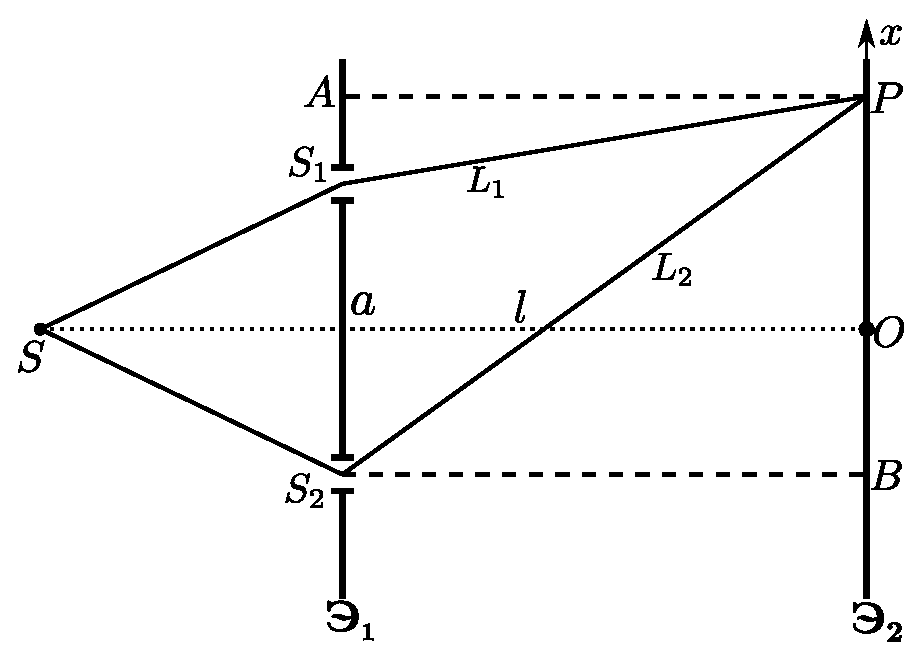
\includegraphics[width=1\linewidth]{img/o-05_1}{}
	\caption{Общая схема наблюдения интерференции}
	\llabel{o-02-scheme}
\end{wrapfigure}

\textbf{Общая схема наблюдения интерференции.}
Световые лучи от источника $S$ проходят через две щели на экране $\text{Э}_1$, образуя два источника $S_1$ и $S_2$. Лучи от этих источников попадают на экран $\text{Э}_2$, на котором наблюдается интерференционная картина в виде плавно переходящих друг в друга светлых полос, перпендикулярных плоскости рисунка.

Из теоремы о когерентности источников при условии, что угол между плоскостями колебаний световых векторов
\footnote{
	векторов напряженности электрических полей электромагнитных волн.
}
достаточно мал, получим:
\begin{gather}
\llabel{o-02-mainint}
I = I_1 + I_2 + 2\sqrt{I_1 I_2}\langle\cos(\Delta \varphi)\rangle
\end{gather}
где $2\sqrt{I_1 I_2}\langle\cos(\Delta \varphi)\rangle$ называется интерференционным членом.

Применим приведенную выше формулу для этой схемы, для этого найдем $\Delta = L_2 - L_1$. Из
$\triangle S_1AP$ и $\triangle S_2BP$ отыщем $L_1$ и $L_2$ (см. Рис. \lref{o-02-scheme}):
$$
L_1 = \sqrt{l^2 + \left(x-\frac{a}{2}\right)^2}, \qquad
L_2 = \sqrt{l^2 + \left(x+\frac{a}{2}\right)^2},
$$
положим $l \gg a, \ l \gg |x|$ и воспользуемся теоремой Тейлора для $L_1$ и $L_2$:
\begin{gather*}
L_1 \approx l + \frac{\left(x-a/2\right)^2}{2l}, \qquad
L_2 \approx l + \frac{\left(x+a/2\right)^2}{2l},
\end{gather*}
тогда
\begin{gather}
\llabel{o-02-schemediff}
\displaystyle \Delta = L_2 - L_1 = \frac{xa}{l}
\end{gather}
Теперь, зная оптическую разность хода, подставим ее в формулу для интенсивности(0.1):
\begin{gather*}
I = I_1 + I_2 + 2\sqrt{I_1 I_2}\cos\left(\frac{2\pi}{\lambda}\Delta\right) =
I_1 + I_2 + 2\sqrt{I_1 I_2}\cos\left(\frac{\pi x a}{\lambda l}\right),
\end{gather*}
для $I_1 = I_2 = I_0$:
\begin{gather}
\llabel{o-02-intensesch}
I = 2I_0\left(1 + \cos\left(\frac{2\pi}{\lambda}\Delta\right)\right) =
4I_0\cos^2\left(\frac{\pi xa}{\lambda l}\right),
\end{gather}

\textit{Интерференция света в тонких плёнках}\\
\begin{figure}[h]
	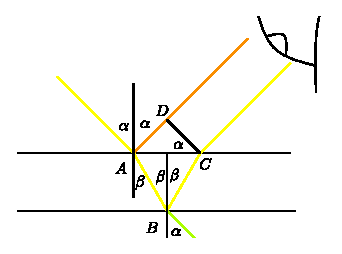
\includegraphics[width=1\linewidth]{img/o-05.eps}
	\caption{Интерференция в тонкой плёнке. $\alpha$ — угол падения, $\beta$ — угол преломления, жёлтый луч отстанет от оранжевого, они сводятся глазом в один и интерферируют.}
\end{figure}
Так, интерференция возникает при разделении первоначального луча света на два луча при его прохождении через тонкую плёнку, например плёнку, наносимую на поверхность линз у просветлённых объективов. Луч света длиной волны $\lambda$ , падая перпендикулярно к поверхности плёнки толщиной $d$, отразится дважды — от внутренней и наружной её поверхностей. Если пленка достаточно тонка, так что её толщина не превышает длину цуга волн падающего света, то на верхней границе раздела сред отражённые лучи будут когерентны и поэтому смогут интерферировать.

Изменение фазы проходящего через плёнку луча, в общем случае, зависит от показателя преломления плёнки и окружающих её сред. Кроме того, надо учитывать, что свет при отражении от оптически более плотной среды меняет свою фазу на половину периода. Так, например, в случае для воздуха ($n_1 ≈ 1$), окружающего тонкую масляную плёнку ($n_2 ≈ 1.5$), луч, отражённый от внешней поверхности будет иметь сдвиг фазы $\pi$ , а от внутренней — не будет. Интерференция будет конструктивной, если итоговая разница между пройденными этими лучами путями на поверхности плёнки будет составлять полуцелое число длин волн в плёнке $\lambda_2 = \lambda_1\frac{n_1}{n_2}$.\\
То есть\\
${\displaystyle \Delta \varphi _{const}=2d{\frac {2\pi }{\lambda _{2}}}+\pi (2k-1)=2d{\frac {2\pi n_{2}}{\lambda _{1}n_{1}}}+\pi (2k-1),k\in \mathbb {Z} }$\\ 
Для деструктивной интерференции в данном примере необходимо, чтобы разность фаз между лучами была кратна $2\pi$ .\\
То есть ${\displaystyle \Delta \varphi _{dest}=2d{\frac {2\pi n_{2}}{\lambda _{1}n_{1}}}+2\pi k,k\in \mathbb {Z} }$ \\
Полное гашение лучей произойдет для толщин пленки:\\
${\displaystyle d_{dest}={\frac {1}{2}}\lambda _{1}k{\frac {n_{1}}{n_{2}}}}$ 
Если ${\displaystyle \lambda _{1}=400}$ нм, то длина этой волны в масляной пленке ${\displaystyle \lambda _{2}=\lambda _{1}{\frac {n_{1}}{n_{2}}}=400{\frac {1}{1.5}}\approx 267}$ нм.

\end{document}